\documentclass[a4paper, 12pt]{article}
\usepackage[total={17cm,25cm}, top=2.5cm, left=2.5cm, right=2.5cm,  includefoot]{geometry}
\usepackage[utf8]{inputenc}
\usepackage{array}
\usepackage{multirow}
\usepackage{hhline}
\usepackage{gensymb}
\usepackage{graphicx}
\graphicspath{ {} }
\usepackage[czech]{babel}
\usepackage{enumitem}
\usepackage{pdfpages}
\usepackage{amsmath}
\usepackage{verbatim}
\usepackage{listings}
\usepackage{hyperref}
\usepackage{amssymb}


\pagestyle{empty} % vypne číslování stránek




\usepackage[OT2,OT1]{fontenc}
\newcommand\cyr
{
\renewcommand\rmdefault{wncyr}
\renewcommand\sfdefault{wncyss}
\renewcommand\encodingdefault{OT2}
\normalfont
\selectfont
}
\DeclareTextFontCommand{\textcyr}{\cyr}
\def\cprime{\char"7E }
\def\cdprime{\char"7F }
\def\eoborotnoye{\char’013}
\def\Eoborotnoye{\char’003}


\begin{document}



\begin{titlepage}
\begin{center}
\noindent
\Large \textbf{České vysoké učení technické v Praze }\\ Fakulta stavební
\vspace{5cm}

\huge

%vložení loga cvut
\begin{figure}[h!]
	\centering
	
\includegraphics[width=7cm]{logo.png}
\end{figure}

\vspace{0.5cm}

Algoritmy v digitální kartografii \\

\vspace{3cm}

\Huge  
Konvexní obálky\\

\vspace{2cm}

\Large
Bc. Robin Pflug \\
Bc. Tomáš Klemsa \\

\end{center}

\end{titlepage}




\pagestyle{plain}     % zapne obyčejné číslování
\setcounter{page}{1}  % nastaví čítač stránek znovu od jedné

\tableofcontents
\newpage

\section{Zadání úlohy}

\textbf{Vstup:} \textit{množina} $P=(p_1,...,p_n),p_i=[x,y_i]$.\\
\textbf{Výstup:} 	\textit{CH(P)}\\

Nad množinou P implementujete následující algoritmy pro konstrukci \textit{CH(P)}:
\begin{itemize}
  \item Jarvis Scan,
  \item Quick Hull,
  \item Sweep Line.
\end{itemize}

Vstupní množiny bodů včetně vygenerovaných konvexních obálek vhodně vizualizujte. Pro množiny n $\epsilon< 1000, 1000000 >$
vytvořte grafy ilustrující doby běhu algoritmů pro zvolená n. Měření proveďte pro různé typy vstupních množin
(náhodná množina, rastr, body na kružnici) opakovaně (10x) a různá n (nejméně 10 množin) s uvedením rozptylu.
Naměřené údaje uspořádejte do přehledných tabulek.
Zamyslete se nad problematikou možných singularit pro různé typy vstupních množin a možnými optimalizacemi.
Zhodnoťte dosažené výsledky. Rozhodněte, která z těchto metod je s ohledem na časovou složitost a typ vstupní
množiny P nejvhodnější.

\subsection{Bonusové úlohy}

Ze zadání bonusových úloh byla řešena konstrukce konvexní obálky metodou \textit{Graham Scan}, kontrukce striktně konvexních obálek , ošetření metody \textit{Jarvis Scan}: existence kolineárních bodů v datasetu a byl vytvořen algoritmus pro automatické generování množin bodů různých tvarů. 

\begin{figure}[h!]
	\centering
	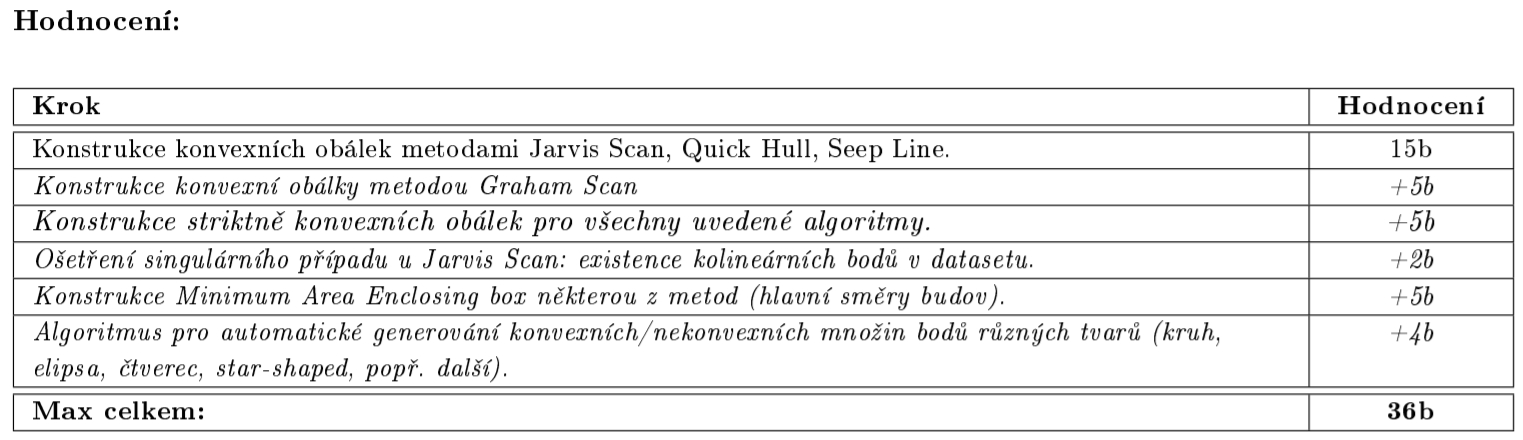
\includegraphics[width=16cm]{hodnoceni.jpg}
	\caption{Bodové hodnocení úlohy [zdroj: 1]}
\end{figure}

\clearpage

\section{Obecná formulace a řešení problému}
\textbf{Definice konvexní obálky:} Konvexní obálka množiny \textit{CH} konečné množiny \textit{S} v $E^2$ představuje nejmenší konvexní mnohoúhelník \textit{P} obsahující \textit{S}.\\
\\
Konvexní obálku si lze představit jako co nejmenší množinu bodů poskládaných tak, že tvoří vrcholy uzavřeného konvexního polygonu. Všechny body zadané množiny se pak nacházejí uvnitř nebo na hraně tohoto polygonu.\\

\begin{figure}[h!]
	\centering
	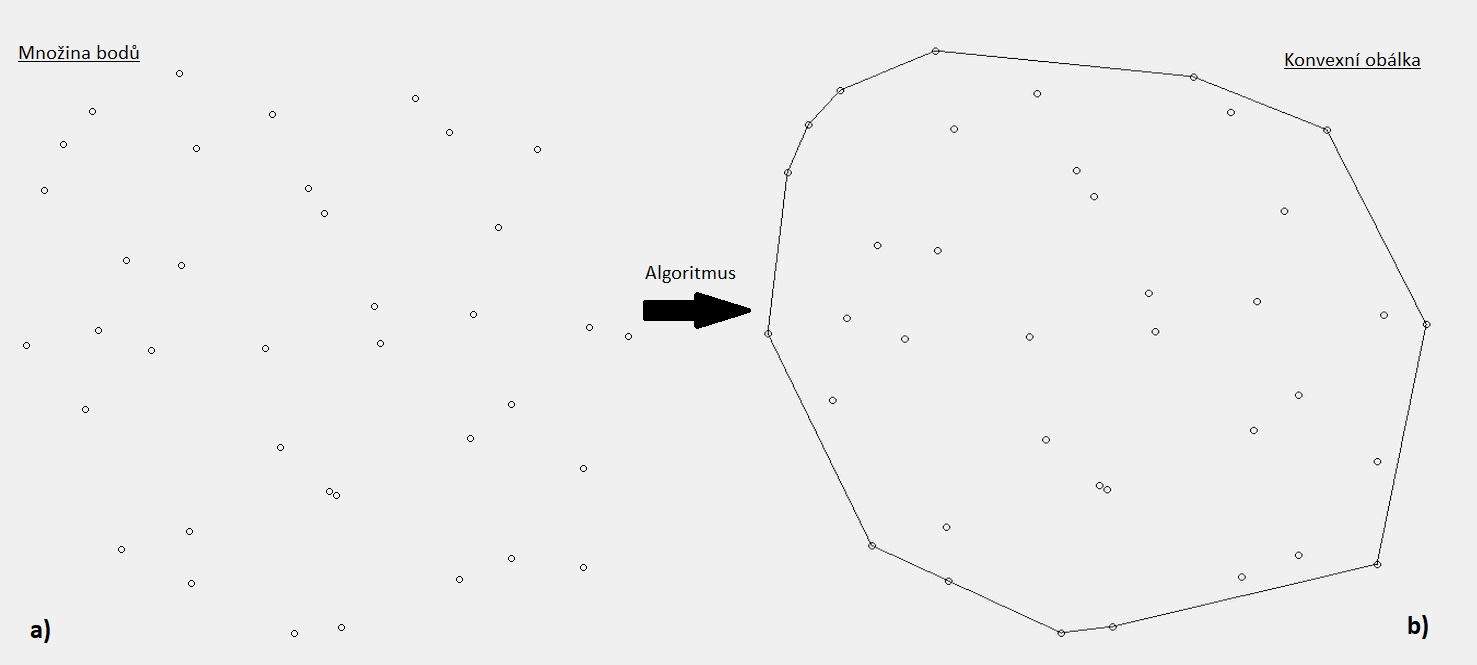
\includegraphics[width=16cm]{convex_hull.jpg}
	\caption{Ukázka množiny bodů, kolem nichž je algoritmem vytvořena konvexní obálka.}
\end{figure}

Zadáním této úlohy bylo vytvořit aplikaci využívající různé algoritmy pro tvorbu konvexních obálek nad zadanou množinou bodů. Dalším cílem úlohy bylo zhodnotit časovou náročnost výpočtů těchto algoritmů nad ruznými množinami bodů. Problematika byla řešena aplikací celkem čtyř algoritmů: Jarvis Scan, Quick Hull, Sweep Line a Graham Scan. Widgedts aplikace byla vytvořena v jazyce C++ na platformě Qt Creator. Aplikace obsahuje funkci pro generování bodů, zpracování bodů a grafický výstup ve formě konvexní obálky i implementaci časové náročnosti jednotlivých algortimů. \\

\section{Aplikované algoritmy}
Algoritmy využívané pro tvorbu konvexní obálky: Jarvis Scan, Quick Hull, Sweep Line, Graham Scan. 

\subsection{Jarvis Scan}
Jednoduchý algoritmus fungující na principu přidávaného bodu, který maximalizuje úhel vzhledem k posledním dvoum bodům obálky. $ p_j+1 = arg\,max_{\forall p_i \in P}  \angle (p_{j-1}, p_j, p_i)$ [zdroj: 1]\\
Algoritmus lze rozšířit do $R^3$. Dataset musí být ošetřen tak, aby neobsahoval tři kolineárních body. Nevýhodou Jarvis Scan algoritmu je složitost $O(n^2)$. Z tohoto faktu vyplývá, že není vhodný pro velké množiny bodů. \\
\\
Prvním krokem při tvorbě konvexní obálky nad množinou bodů metodou Jarvis Scan je nalezení pivota \textit{q}. Jako pivot se určí takový bod ze zadané množiny, který má nejmenší souřadnici \textit{y}. Nalezený bod, určený jako pivot \textit{q}, bude prvním bodem konvexní obálky. \\
Dalším krokem je inicializace takového bodu \textit{r}, který tvoří s bodem \textit{q} rovnoběžku s osou \textit{y}.
Po nalezení pivotu a bodu \textit{r} budu provádět cyklicky hledání bodu, který má vzhledem k zadané přímce, tvořené posledními dvěmi body konvexní obálky, maximální úhel (v prvním kroku tohoto cyklu se jako poslední dva body obálky uvažijí \textit{r} a \textit{q}. Pokud je takový bod nalezen, přidám tento bod do konvexní obálky a opakuji tento cyklus. Cyklus končí v momentě, kdy je jako přidávaný bod vyhodnocen bod \textit{q}.\\

\begin{figure}[h!]
	\centering
	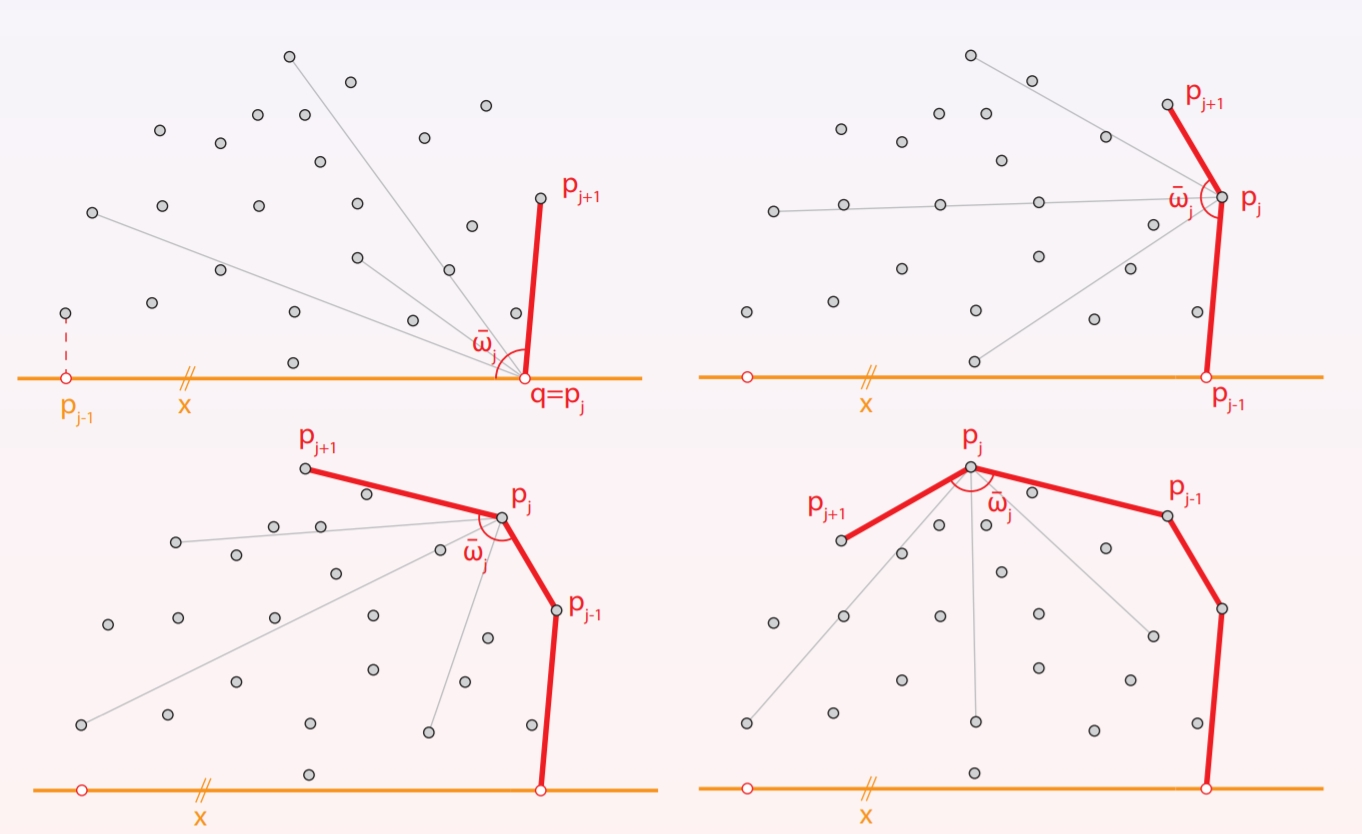
\includegraphics[width=12cm]{jarvis.jpg}
	\caption{Jarvis Scan algoritmus [zdroj: 1]}
\end{figure}

\subsubsection{Algoritmus Jarvis Scan}
\begin{enumerate}
\item Nalezení pivota q,$ q = min(y_i) $ 
\item Přidej $ q \rightarrow CH  $ 
\item Inicializuj: $p_j = q; p_{j+1} = p_{j-1}$
\item Opakuj, dokud $ p_{j+1} \ne q $
\subitem Nalezni $p_{j+1}$: $ p_{j+1} = arg  max_{\forall p_i \in P}  \angle (p_{j-1}, p_j, p_i)$
\subitem Přidej $p_{j+1}$: $ p_{j+1} \rightarrow H  $
\subitem $ p_{j-1} = p_j; p_j = p_{j+1}  $
\end{enumerate}[zdroj: 1]


\subsection{Quick Hull}
Algoritmus pro tvorbu konvexní obálky metodou Quick Hull využívá strategie Divide and Conquer. Ve většině případů funguje rychle s časovou naročností (n log n), ovšem při špatném rozložení bodů v datasetu dosahuje časové náročnosti ($n^2$). Rychlé provedení algoritmu je podmíněno malým počtem rekurzivních kroků. Při tvorbě expanduje konvexní obálka všemi směry. \\
\\
Prvník krokem pro tvorbu kovexní obálky touto metodou je setřídění bodů datasetu podle velikosti souřadnice \textit{$x_i$}. Z takto setříděných bodů vyberu jeden \textit{$q_1$} s minimální souřadnicí \textit{$x$} a druhý \textit{$q_3$} s maximální souřadnicí \textit{$x$}.
Tyto dva body \textit{$q_1$} a \textit{$q_3$} rozdělí rovinu s množinou bodů na horní a dolní polorovinu. Takto vzniklé poloroviny s množinou bodů jsou zpracovávány samostatně. V polorovině je volána rekurzivně lokální procedura. Ta určí jako bod konvexní obálky takový, který je od zadané přímky dané počátečním a koncovým vrcholem nejdále.

\begin{figure}[h!]
	\centering
	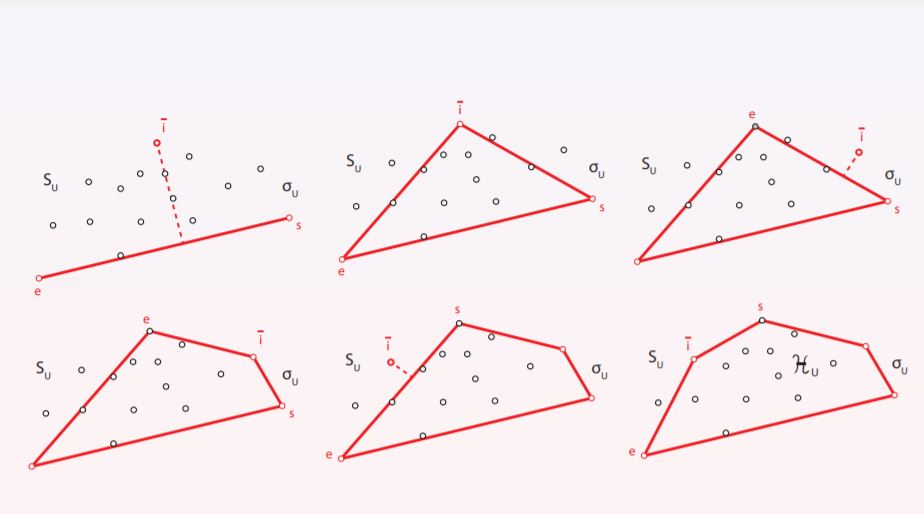
\includegraphics[width=12cm]{quickhull.jpg}
	\caption{Princip Quick Hull algoritmu [zdroj: 1]}
\end{figure}

\newpage
\subsubsection{Algoritmus Quick Hull globální metoda}
\begin{enumerate}
\item $CH = 0; S_U = 0; S_L = 0 $ 
\item $ q_1 =  min_{\forall p_i \in S}(x_i); q_3 =  max_{\forall p_i \in S}(x_i) $ 
\item $S_U \leftarrow q_1; S_U \leftarrow q_3; S_L \leftarrow q_1; S_L \leftarrow q_3 $
\item for $\forall p_i \in S  $
\subitem  if$ (p_i \in \sigma_l(q_1, q_3)) S_U \leftarrow p_i  $
\subitem else $ S_L \leftarrow p_i  $
\item $CH \leftarrow q_3$
\item Nalezení nejvzdálenějšího bodu $c$ v horní části od přímky, přidání do množiny konvexní obálky a opakování vůči nově vzniklé přímce.
\item $CH \leftarrow q_1$
\item Opakování hledání nejvzdálenějšího bodu v dolní části.
\end{enumerate}
[zdroj: 1]
\newpage
\subsection{Sweep line}
Tvorba konvexní obálky metodou Sweep line využívá inkrementální konstrukci.\\ Princip inkrementální konstrukce je založen na přidávání bodů do konvexní obálky po jednom. Tvar konvexní obálky je tudíž postupně modifikován.\\
V metodě Sweep line je rovina rozdělena na zpracovanou a nezpracovanou část. Složitost algoritmu je (n log n) a lze jej převést do vyšší dimezne. Nevýhodou je citlivost vůči duplicitním bodům.\\
\\
Prvním krokem algoritmu Sweep line je setřídění celé množiny bodu podle velikosti souřadnice \textit{x}. Dále algoritmus určí jako iniciální řešení dvojúhelník (trojúhelník) tvořený prvními dvěma (třema) body setříděného datasetu. Po přidání dalšího bodu je konvexní obálka updatována a dále expanduje v kladném směru osy \textit{x}. 

\begin{figure}[h!]
	\centering
	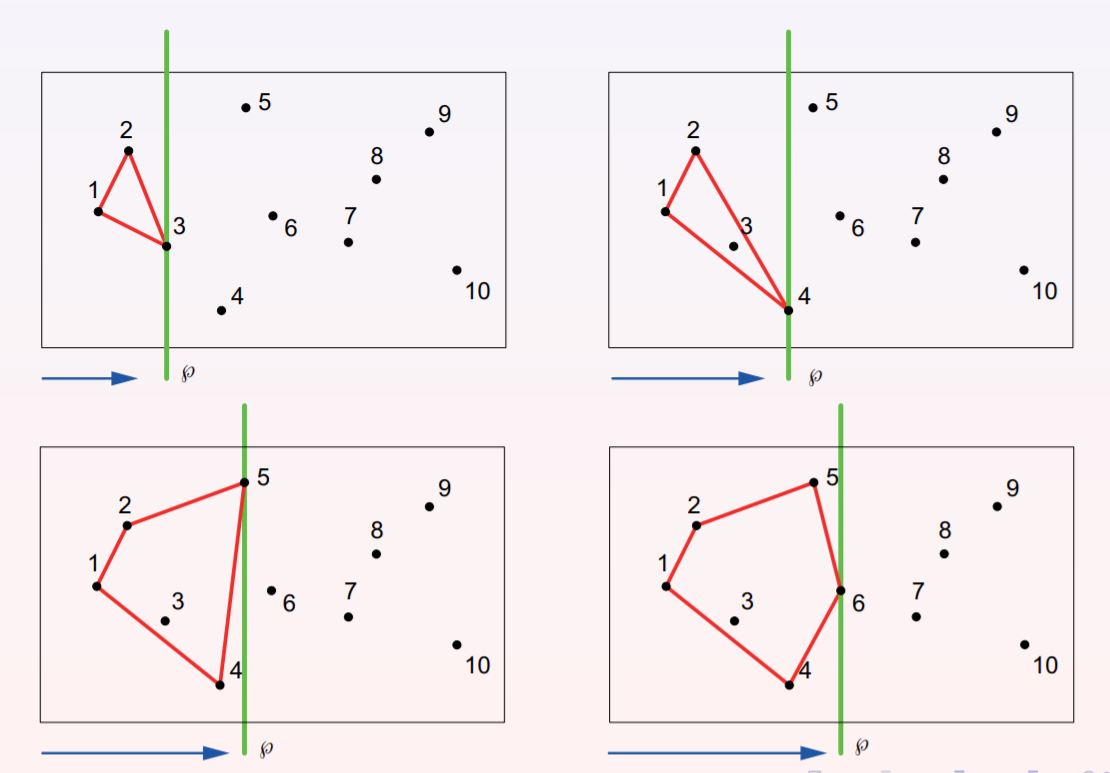
\includegraphics[width=12cm]{sweep_line.jpg}
	\caption{Sweep line [zdroj: 1]}
\end{figure}

\newpage
\subsubsection{Algoritmus Sweep line}
\begin{enumerate}
\item $ Sort P_s = sort(P) ~by~ x $ 
\subitem Změna indexů následovníků: $ n[0] = 1; n[1] = 0  $
\subitem Změna indexů předchůdců: $ p[0] = 1; p[1] = 0$
\item $ for~ p_i \in P_S, i \textgreater 1$
\subitem $ if (y_i \textgreater y_{i-1})  $
\subsubitem $ p[i] = i-1; n[i] = n[i-1]$
\item else $ p[i] = p[i-1]; n[i] = i-1$
\subitem $ n[p[i]] = i; p[n[i]] = i  $
\subitem $ while (n[n[i]]) \in \sigma_R (i, n[i])  $
\subsubitem Změna indexů: $ p[n[n[i]]] = i; n[i] = n[n[i]]$
\subitem $ while (p[p[i]]) \in \sigma_L (i, p[i])  $
\subsubitem Změna indexů: $ n[p[p[i]]] = i; p[i] = p[p[i]]$
\end{enumerate}
[zdroj: 1]
\newpage
\subsection{Graham Scan}
Algortimus je založen na převodu star-shaped polygonu na konvexní obálku. Převod je realizován za pomoci kritéria levotočivosti. Metodu lze provádět i v $R^3$ a časová složitost je (n log n). Lze tedy říci, že algoritmus je vhodný pro rozsáhlé datasety.\\
\\
Pro konstrukci konvexní obálky metodou Graham Scan je nutné v prvním kroku určit pivota \textit{q} s takovou vlastností, že má nejmenší souřadnici \textit{y} z celé zadané možiny bodů. Další krok je setřídění ostatních bodů datasetu podle velikostu úhlu daného rovnoběžkou s osou \textit{x} procházející bodem \textit{q} a přímkou danou hodnoceným bodem a bodem \textit{q}. Poté jsou z datasetu odstraněny body o stejném úhlu. Odstraněn je bod ležící blíže bodu \textit{q}. Bod \textit{q} a bod o největším úhlu jsou zařazeny do konvexní obálky. Poté cyklicky procházím polohu bodu ze seřazené množiny a hodnotím jeho polohu vůči lini tvořené posledníma dovouma bodama v CH. Poku se nachází přidávaný bod vlevo od linie, je do konvexní obálky přidán. Dále se opakuje cyklus pro další bod ze seřazené množiny. \\
Pokud bod leží vpravo od linie, je poslední bod CH odebrán a cyklus se opakuje. 

\begin{figure}[h!]
	\centering
	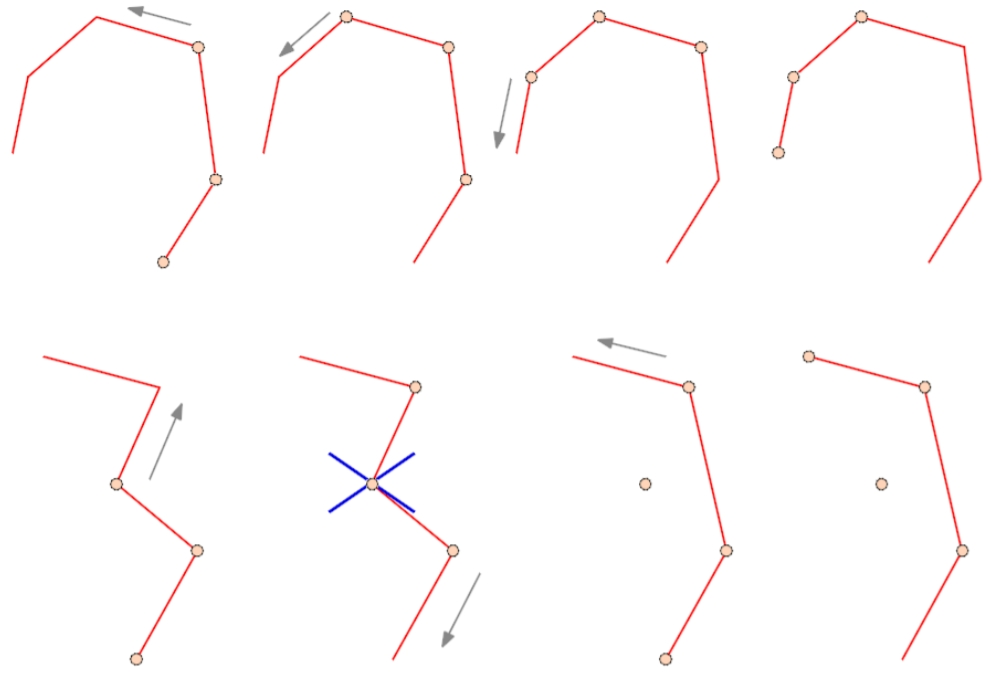
\includegraphics[width=10cm]{graham_scan.jpg}
	\caption{Princip vyhodnocení polohy bodu v metodě Graham Scan [zdroj: 6]}
\end{figure}

\subsubsection{Algoritmus Graham Scan}
\begin{enumerate}
\item $ q = min_{\forall p_i \in S} (y_i), q \in H $ 
\item $ {\forall p_i \in S}$ sort by $ \omega_i = \angle (p_i, q, x)$
\item $ \omega_k = \omega_l \rightarrow $ odstraň bod blíže q 
\item $ H \leftarrow q; H \leftarrow p_1$
\item $ for j < n $
\item if $ p_j $ vpravo od předešlých bodů $ \rightarrow pop S$
\item else $ p_{j}  \rightarrow H $
\end{enumerate}
[zdroj: 1]
\section{Bonusové úlohy}

\subsection{Konstrukce konvexní obálky metodou Graham Scan}
Řešení této úlohy je popsáno v kapitole Aplikované algoritmy - Graham Scan.

\subsection{Konstrukce striktně konvexních obálek}
Striktně konvexní obálky jsou takové, že po sobě následující 3 body neleží na stejné přímce. Striktně konvexní obálky byly tvořeny ve funkci \textit{strictlyConvex}. Tato funkce příjmá na vstupu klasickou konvexní obálku ve formě polygonu. Z polygonu jsou nejprve odstraňovány duplicitní body. Poté je kontrolováno, zda tři po sobě jdoucí body neleží na stejné přímce. Pokud ano, prostřední bod je odstraněn z konvexní obálky.

\subsection{Jarvis Scan: existence kolineárních bodů v datasetu}
Pokud vstupní množina bodů obsahuje kolineární body, mohla by nastat situace kdy bod \textit{k} má stejný úhel jako jiný bod \textit{l} vzhledem ke stejné přímce $\angle (p_j-1, p_j, p_k)=(p_j-1, p_j, p_l)$. Pro ošetření tohoto případu byla přidána podmínka pro stejné úhly, která do konvexní obálky přidá z takovéto dvojice bodů ten, který je od bodu $p_j$ vzdálenější. 

\subsection{Automatické generování množin bodů}

Uživetal ve spodní části ovládacího panelu má možnost generovat náhodně body. V rozbalovacím seznamu může vybrat z položek Circle, Square, Random a Raster a ve spinboxu může zvolit počet generovaných bodů od 10 do 1000000. Tlačítkem generate points se body přidají do Okna.

\section{Vstup dat do aplikace}
Vstup dat v aplikaci lze realizovat dvěma způsoby. Uživatel sám vkládá body do grafického okna za pomoci kurzoru myši nebo vygeneruje náhodné body funkcemi z kapitoly \textit{Bonusové úlohy - Automatické generování množin bodů}.

\section{Výstup aplikace}
Výstupem grafického rozhraní aplikace je uzavřený polygon konvexní obálky vytvořený zadanou metodou nad vstupní množinou bodů. Další částí výstupu je časová náročnost výpočtu daného algoritmu pro aktuální množinu bodů v datasetu. 

\section{Dokumentace}
\subsection{Třídy}
\subsubsection{Algorithms}
Třída Algorithms obsahuje metody zajišťující výpočty daných algoritmů.
\\

\textbf{double getPointLineDistance(QPoint q, QPoint p1, QPoint p2)}\\
Návratová hodnota: \textit{double};\\
Metoda vrátí vzdálenost bodu \textit{q} od přímky dané body\textit{ p1} a \textit{p2}.
\\

\textbf{int getPointLinePosition(QPoint q,QPoint p1,QPoint p2)}\\
Návratová hodnota: \textit{integer};\\
Metoda vrátí polohu bodu \textit{q} vůči přímce dané body\textit{ p1} a \textit{p2}. Hodnota 1 je pro polohu vlevo od přímky, 0 pro polohu vpravo od přímky a -2 pro polohu bodu na přímce.
\\

\textbf{double getAngle2Vectors(QPoint p1,QPoint p2,QPoint p3,QPoint p4)}\\
Návratová hodnota: \textit{double};\\
Metoda vrátí úhel mezi přímkou zadané body p1, p2  a přímkou zadané body p3 a p4.
\\

\textbf{QPolygon strictlyConvex(QPolygon ch)}\\
Návratová hodnota: \textit{QPolygon};\\
Metoda ze zadané obecné konvexní obálky ve formě polygonu vytvoří striktně konvexní obálku a vrátí jí ve formě polygonu.
\\

\textbf{QPolygon jarvisScan(std::vector$<QPoint>$ points)}\\
Návratová hodnota: \textit{QPolygon};\\
Metoda z vektoru bodů vytvoří striktně konvexní obálku ve formě polygonu metodou Jarvis Scan. 
\\

\textbf{QPolygon qHull(std::vector$<QPoint>$ points)}\\
Návratová hodnota: \textit{QPolygon};\\
Metoda z vektoru bodů vytvoří striktně konvexní obálku ve formě polygonu metodou Quick Hull. 
\\

\textbf{void qh(int s, int e, std::vector$<QPoint>$ points, QPolygon ch)}\\
Návratová hodnota: \textit{Void};\\
Pomocná metoda k výpočtu konvexní obálky metodou Quick Hull. 
\\

\textbf{QPolygon sweepLine(std::vector$<QPoint>$ points)}\\
Návratová hodnota: \textit{QPolygon};\\
Metoda z vektoru bodů vytvoří striktně konvexní obálku ve formě polygonu metodou Sweep line. 
\\

\textbf{QPolygon grahamScan(std::vector$<QPoint>$ points)}\\
Návratová hodnota: \textit{QPolygon};\\
Metoda z vektoru bodů vytvoří striktně konvexní obálku ve formě polygonu metodou Graham Scan. 
\\

\subsubsection{SortbyX}
Třída SortbyX slouží k porovnání souřadnic v ose x.\\


\textbf{bool operator()(QPoint \&p1, QPoint \&p2)}\\
Přetížený operátor () vrátí bod s větší souřadnicí x z dvojice bodů.\\


\subsubsection{SortbyY}
Třída SortbyY slouží k porovnání souřadnic v ose y.
\\

\textbf{bool operator()(QPoint \&p1, QPoint \&p2)}\\
Přetížený operátor () vrátí bod s větší souřadnicí y z dvojice bodů.
\\

\subsubsection{sortPointsAngleQ}
Třída sortPointsAngleQ obsahuje funkci pro seřazení bodů vzhledem k rovnoběžce s osou \textit{x} procházející bodem \textit{q}.

\textbf{std::vector$<QPoint>$ sortPointsByAngleQ (std::vector$<QPoint>$ points, QPoint q)}\\
Návratová hodnota: \textit{vector$<QPoint>$};\\
Metoda metoda vrátí vektor bodů, které jsou seřazeny podle velikosti úhlu mezi rovnoběžkou s osou \textit{x} vedenou bodem \textit{q} a přímkou danou bodem \textit{q} a hodnoceným bodem.

\newpage
\section{Testování}
Pro každou množinu bodů bylo provedeno 10 testů, výsledný čas uvedený v tabulkách je průměrem časů těchto testů.

\subsection{Jarvis Scan}

\begin{figure}[h!]
	\centering
	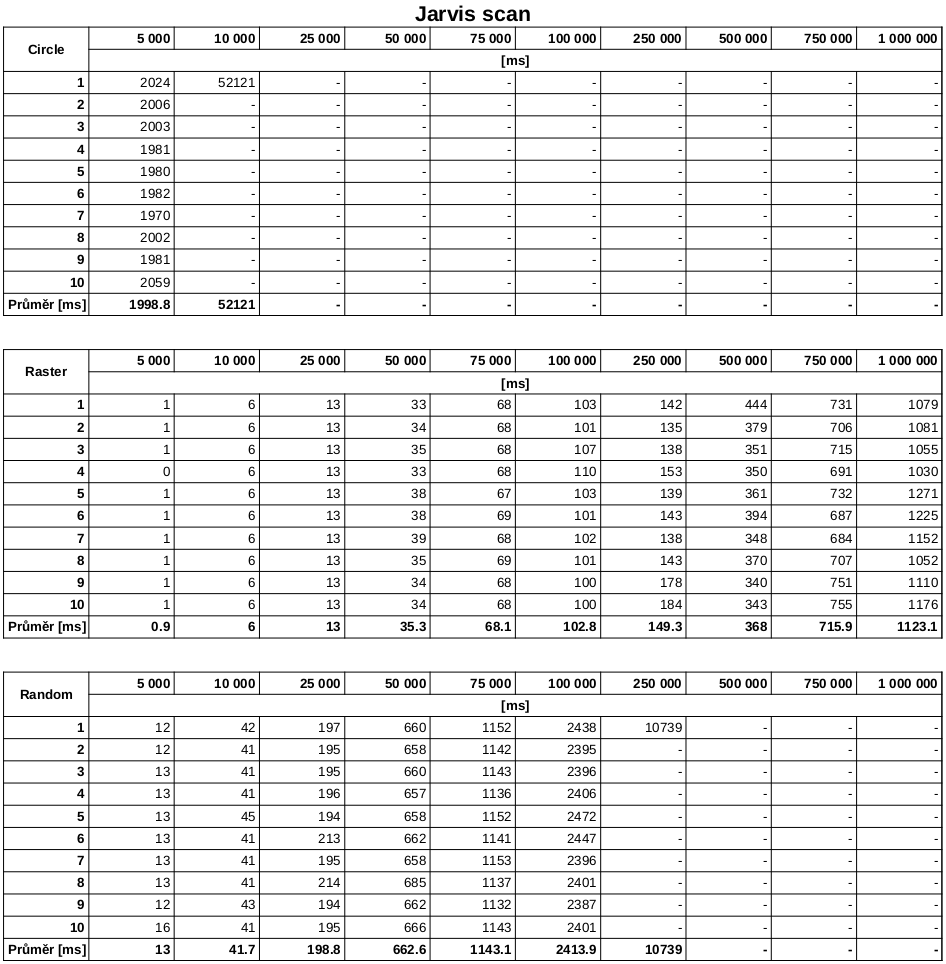
\includegraphics[width=10cm]{data_jarvis_scan.png}
	\caption{Testování časové náročnosti Jarvis Scan}
\end{figure}

\begin{table}[h!]
	\centering
	\begin{tabular}{|r|r|r|r|}
	\hline
	 \textbf{Počet bodů} 	& \textbf{Circle [ms]} & \textbf{Rastr [ms]}  & \textbf{Random [ms]} \\ \hline
	 5000 & 79.1 & 0.9 & 13   \\ \hline
	10000 & 1998.8 & 6 & 13   \\ \hline
	25000 & 21482.2 & 13 & 198.8  \\ \hline
	50000 & 55892.4 & 35.3 & 662.6   \\ \hline
	75000 & 92519 & 68.1 & 1143.1 \\ \hline
	100000 & 133729 & 102.8 & 2413.9  \\ \hline
	250000 & 336309 & 149.3 & 10739   \\ \hline
	500000 & 610392 & 368 & X  \\ \hline
	750000 & X & 715.9 & X  \\ \hline
	1000000 & X & 1123.1 & X  \\ \hline
	
	\end{tabular}
		\caption{Jarvis Scan}
\end{table}

\begin{figure}[h!]
	\centering
	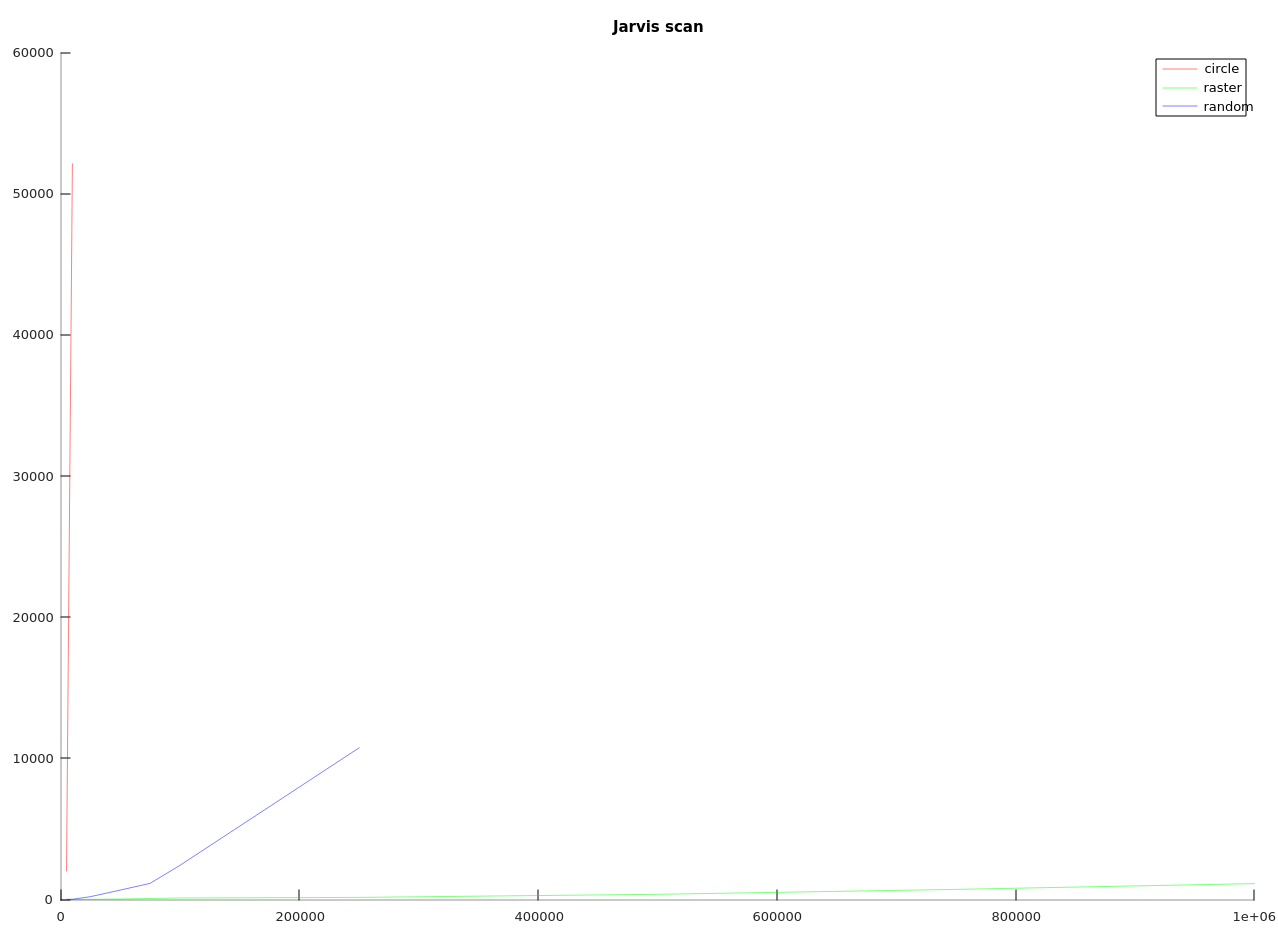
\includegraphics[width=10cm]{figure_jarvis_scan.png}
	\caption{Testování časové náročnosti Jarvis Scan - graf}
\end{figure}

\newpage
\subsection{Sweep Line}

\begin{figure}[h!]
	\centering
	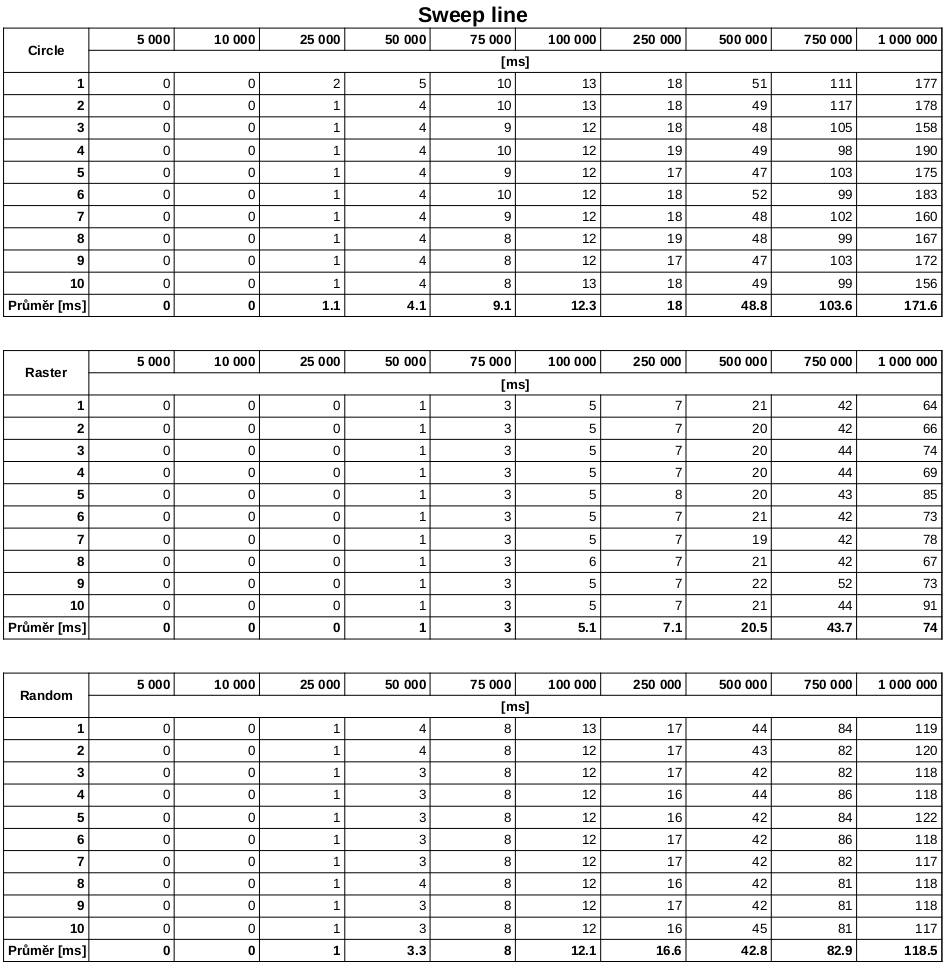
\includegraphics[width=10cm]{data_sweep_line.png}
	\caption{Testování časové náročnosti Sweep Line}
\end{figure}

\begin{table}[h!]
	\centering
	\begin{tabular}{|r|r|r|r|}
	\hline
	 \textbf{Počet bodů} 	& \textbf{Circle [ms]} & \textbf{Rastr [ms]}  & \textbf{Random[ms]} \\ \hline
	 5000 & 0 & 0 & 0   \\ \hline
	10000 & 0 & 0 & 0   \\ \hline
	25000 & 1.1 & 0 & 1  \\ \hline
	50000 & 4.1 & 1 & 3.3   \\ \hline
	75000 & 9.1 & 3 & 8  \\ \hline
	100000 & 12.3 & 5.1 & 12.1  \\ \hline
	250000 & 18 & 7.1 & 16.6   \\ \hline
	500000 & 48.8 & 20.5 & 42.8  \\ \hline
	750000 & 103.6 & 43.7 & 82.9  \\ \hline
	1000000 & 171.6 & 74 & 118.5  \\ \hline
	
	\end{tabular}
		\caption{Sweep Line}
\end{table}

\begin{figure}[h!]
	\centering
	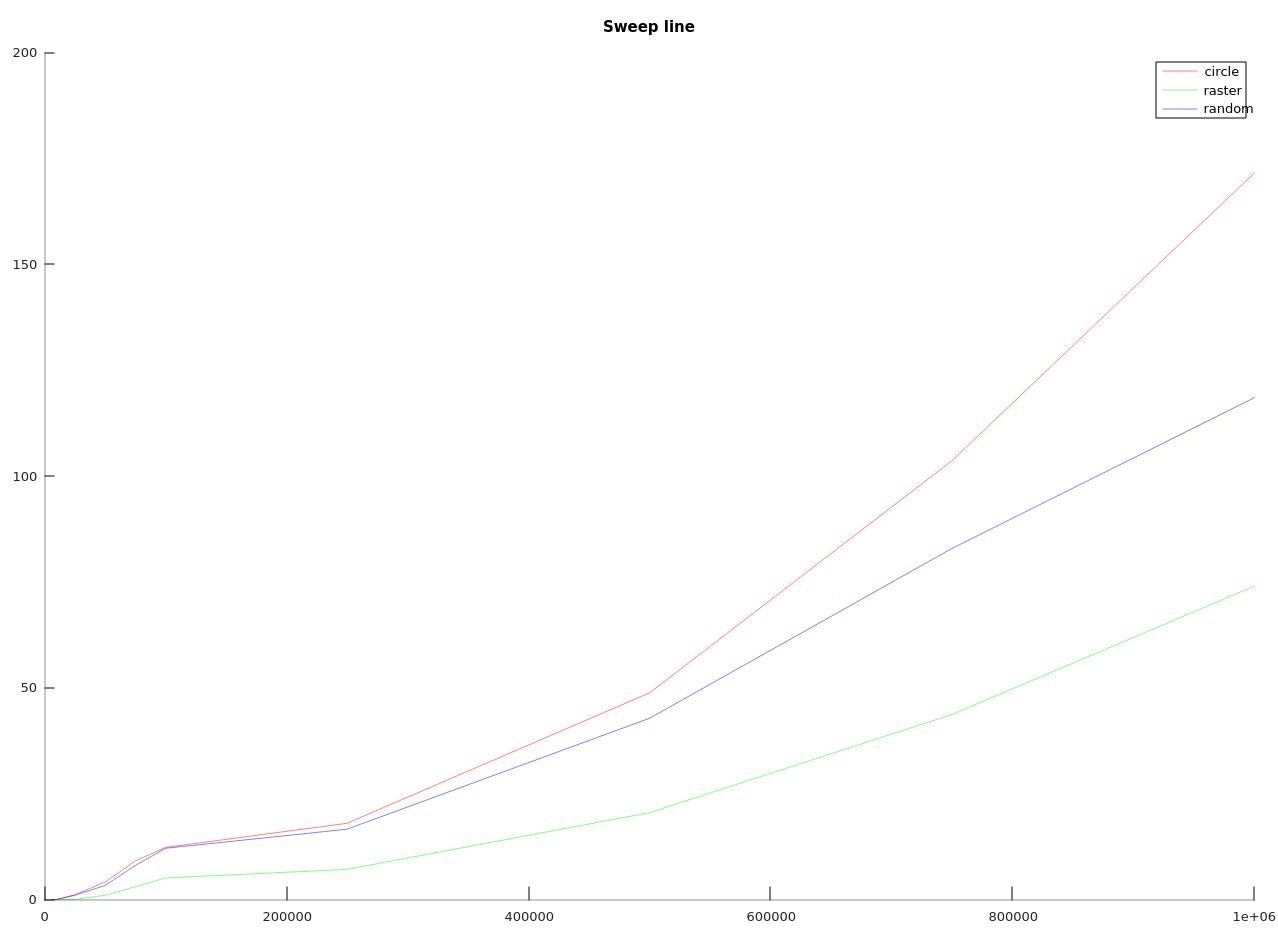
\includegraphics[width=10cm]{figure_sweep_line.png}
	\caption{Testování časové náročnosti Sweep Line - graf}
\end{figure}

\clearpage

\subsection{Quick Hull}

\begin{figure}[h!]
	\centering
	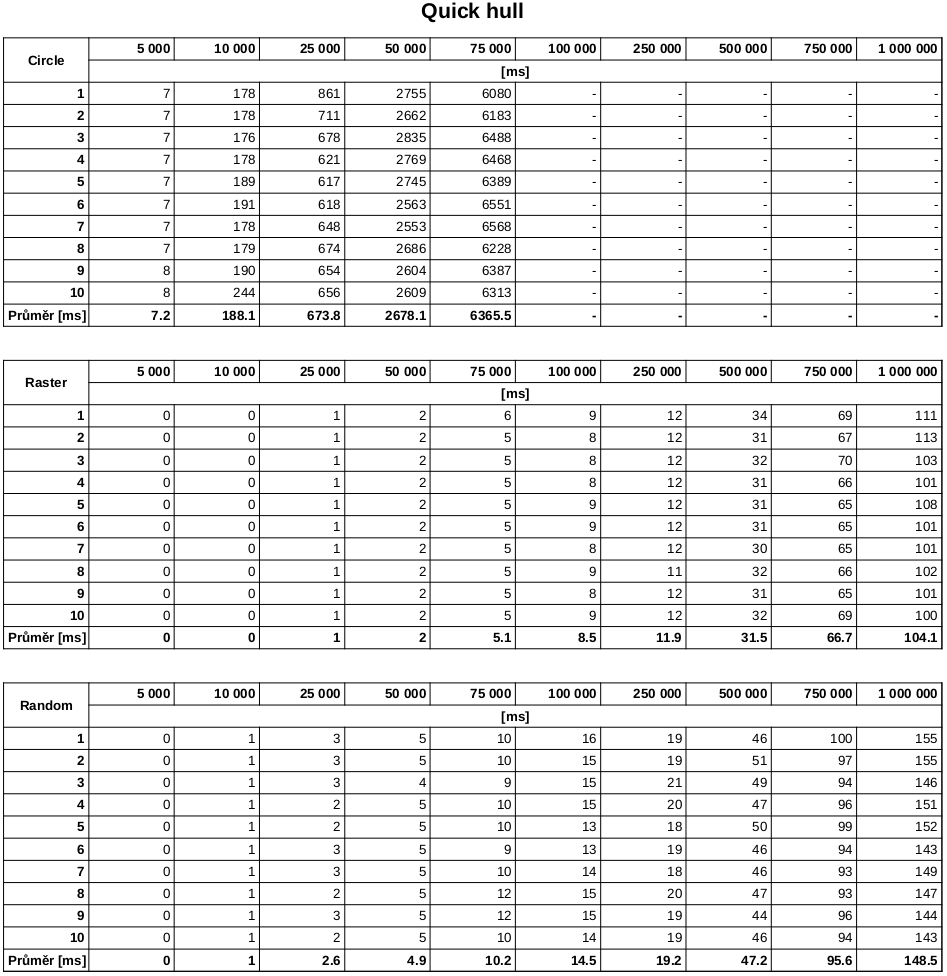
\includegraphics[width=10cm]{data_quick_hull.png}
	\caption{Testování časové náročnosti Quick Hull}
\end{figure}

\begin{table}[h!]
	\centering
	\begin{tabular}{|r|r|r|r|}
	\hline
	 \textbf{Počet bodů} 	& \textbf{Circle [ms]} & \textbf{Rastr [ms]}  & \textbf{Random[ms]} \\ \hline
	 5000 & 7.2 & 0 & 0   \\ \hline
	10000 & 188.1 & 0 & 0   \\ \hline
	25000 & 673.8 & 1 & 2.6  \\ \hline
	50000 & 2678.1 & 2 & 4.9   \\ \hline
	75000 & 6365.5 & 5.1 & 10.2  \\ \hline
	100000 & X & 8.5 & 14.5  \\ \hline
	250000 & X & 11.9 & 19.2   \\ \hline
	500000 & X & 31.5 & 47.2  \\ \hline
	750000 & X & 66.7 & 95.6  \\ \hline
	1000000 & X & 104.1 & 148.5 \\ \hline
	
	\end{tabular}
		\caption{Quick Hull}
\end{table}

\begin{figure}[h!]
	\centering
	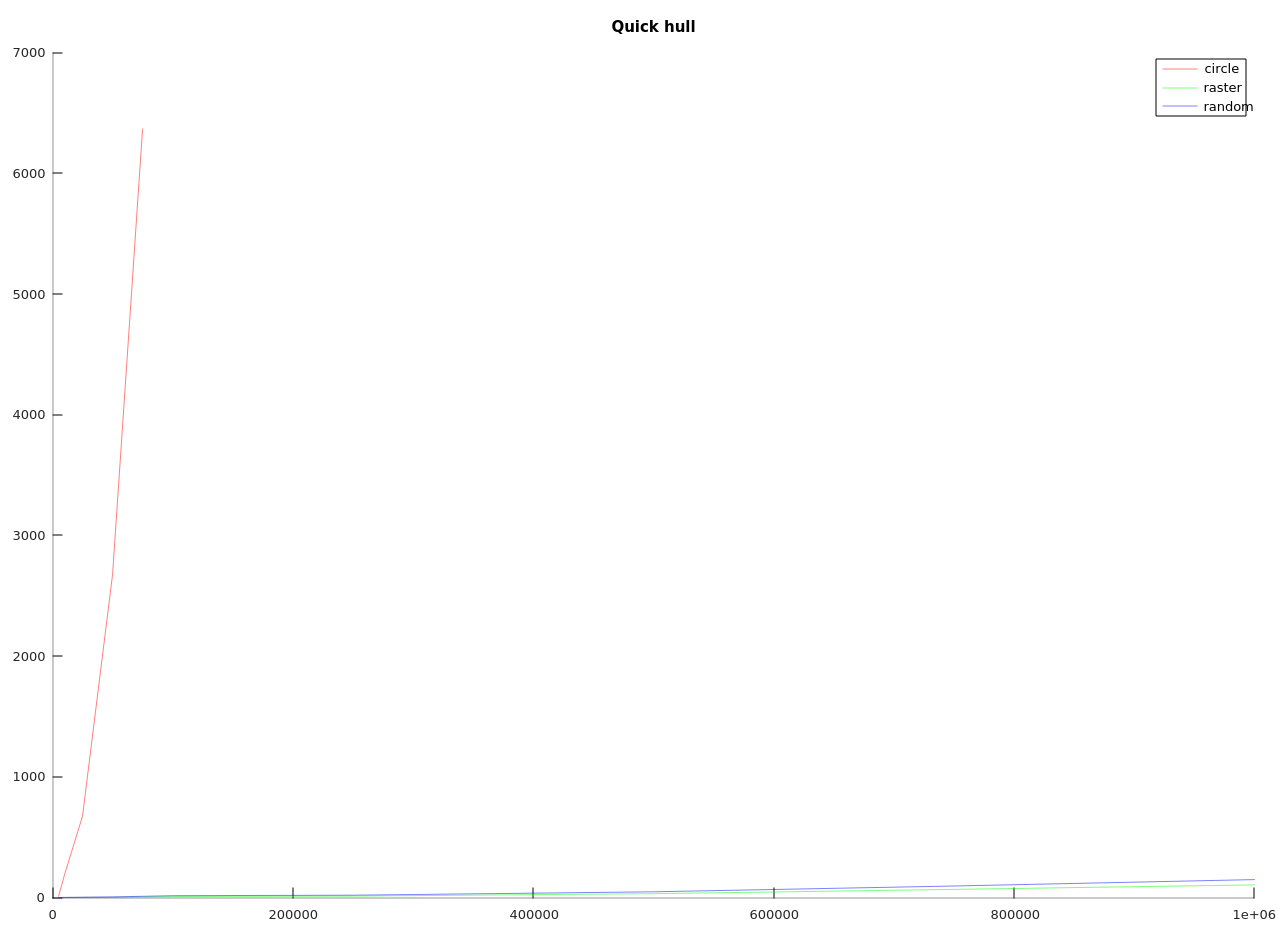
\includegraphics[width=10cm]{figure_quick_hull.png}
	\caption{Testování časové náročnosti Quick Hull - graf}
\end{figure}

\clearpage
\section{Závěr}
Pro tvorbu konvexních obálek byly vytvořeny tři základní metody (Jarvis Scan, Quick Hull, Sweep Line) a jedna bonusová (Graham Scan). Pro nízký počet vstupních bodů fungují všechny algoritmy bez problému. Problémové situace jsou z velké části ošetřeny (duplicitní body apod.). Pro větší množinu vstupních bodů se bez problému podařilo tvořit konvexní obálku pouze metodou Sweep Line. Metoda Jarvis Scan pro náhodně generované body na kružnici v počtu nad 100000 "běží" velmi dlouho, problém se nepodařilo odhalit. Metoda Quick Hull je ze své podstaty nevhodná pro tvorbu konvexní obálky s body na kružnici. Časová náročnost algoritmů pro zadané množiny bodů jsou obsahem předchozí kapitoly Testování. Algoritmus Graham Scan pro malé množství bodů funguje bezchybně, ovšem pro vygenerované větší množství bodů také kolabuje. Tato chyba je nejspíše důsledkem složitosti funkce pro řazení bodů podle úhlu.

\section{Náměty pro vylepšení} 
Pro zlepšení testování algoritmů by bylo výhodné udělat aplikaci výcevláknovou aby bylo vidět že aplikace provádí výpočty a UI se nestalo neaktivní.

\section{Reference}

\begin{enumerate}

\item  BAYER, Tomáš. Metody konstrukce konvexní obálky [online][cit. 5.11.2019]. \\
Dostupné z: https://web.natur.cuni.cz/~bayertom/images/courses/Adk/adk4.pdf  \\

\end{enumerate}
\end{document}



 